        \p
یک جدول مستطیل‌شکل در نظر بگیرید که خانه‌های آن سیاه و سفید شده باشند و در هر سطر و در هر ستون بیش از
$\frac{3}{4}$
خانه‌ها هم‌رنگ باشند. فرض کنید در
$a$
سطر و
$c$
ستون تعداد خانه‌های سفید و در 
$b$
سطر و
$d$
ستون تعداد خانه‌های سیاه بیش‌تر باشد. با جابه‌جایی سطرها و ستون‌ها فرض می‌کنیم در
$a$
سطر بالا و
$c$
ستون سمت چپ جدول تعداد خانه‌های سفید بیش‌تر باشد. طبق فرض تعداد خانه‌های سفید و همچنین تعداد خانه‌های سیاه جدول برابر
$\frac{1}{2}(a + b)(c + d)$ 
است. فرض کنید
$A$
مجموعه‌ی خانه‌های سفید
$a$
سطر بالا و
$B$
مجموعه‌ی خانه‌های سفید
$c$
ستون سمت چپ جدول باشد، در این صورت:
$$\frac{1}{2}(a + b)(c + d) \geq |A \cup B| = |A| + |B| - |A \cap B| >$$
$$\frac{3}{4}a(c + d) + \frac{3}{4}c(a + b) - ac$$
\begin{center}
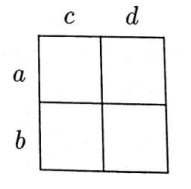
\includegraphics[height=6.5cm]{1.png}
\end{center}
پس از ساده کردن این نابرابری نتیجه می‌گیریم
$2bd > ad + bc$
. از بحث مشابه در مورد خانه‌های سیاه نتیجه می‌گیریم
$2ac > ad + bc$
. حال از ضرب این دو نابرابری نتیجه می‌گیریم:
$$4abcd > (ad + bc)^2 \Rightarrow (ad + bc)^2 - 4abcd < 0$$
$$\Rightarrow (ad - bc)^2 < 0$$
از تناقض حاصل نتیجه می‌گیریم پاسخ مسئله خیر است.       